\documentclass[crop,tikz]{standalone}
\usepackage{circuitikz}
\begin{document}
    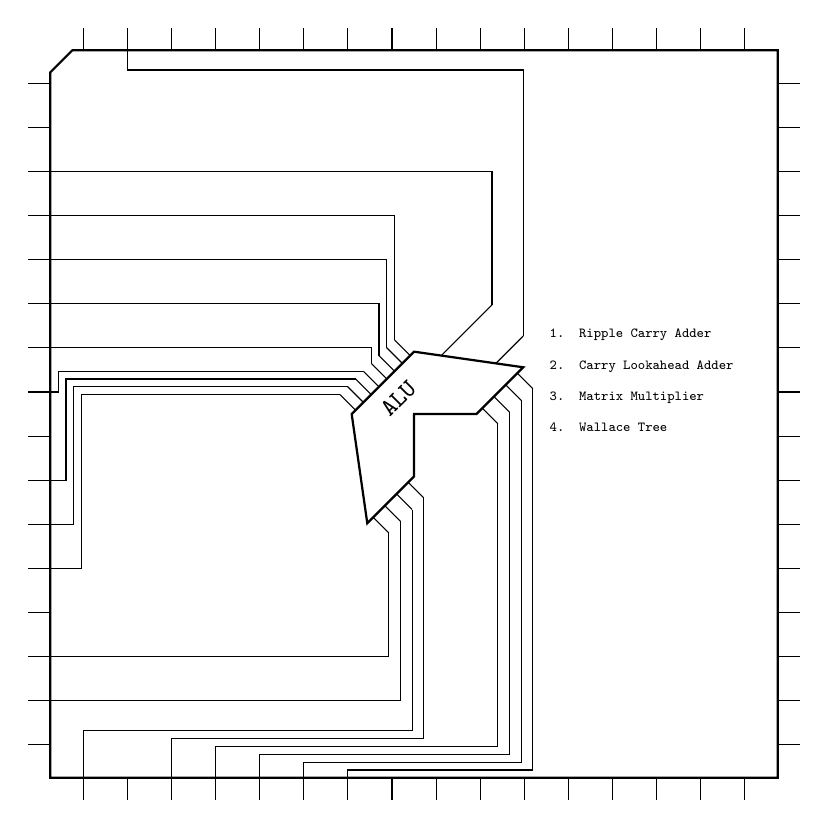
\begin{tikzpicture}
        \draw (0,0) node[qfpchip, num pins=64, hide numbers](C){};
        %
        \tikzset{ALU/.style={muxdemux, muxdemux def={Lh=5, NL=8, Rh=2, NR=8, NB=2, NT=0, w=2, inset w=1, inset Lh=2, inset Rh=0, square pins=1}}}
        \draw (C.center) node[ALU, rotate=135 , scale=1](A){\rotatebox {-90}{\small \ttfamily ALU}};
        %
        \draw (C.bpin 23) -- ++(0,0.10) -| (A.lpin 8);
        \draw (C.bpin 22) -- ++(0,0.20) -| (A.lpin 7);
        \draw (C.bpin 21) -- ++(0,0.30) -| (A.lpin 6);
        \draw (C.bpin 20) -- ++(0,0.40) -| (A.lpin 5);
        %
        \draw (C.bpin 19) -- ++(0,0.50) -| (A.lpin 4);
        \draw (C.bpin 17) -- ++(0,0.60) -| (A.lpin 3);
        \draw (C.bpin 15) -- ++(0,0.00) -| (A.lpin 2);
        \draw (C.bpin 14) -- ++(0,0.00) -| (A.lpin 1);
        %
        \draw (C.bpin  4) -- ++(0,0.00) -| (A.rpin 8);
        \draw (C.bpin  5) -- ++(0,0.00) -| (A.rpin 7);
        \draw (C.bpin  6) -- ++(0,0.00) -| (A.rpin 6);
        \draw (C.bpin  7) -- ++(0,0.00) -| (A.rpin 5);
        \draw (C.bpin  8) -- ++(0.10,0) |- (A.rpin 4);
        \draw (C.bpin 10) -- ++(0.20,0) |- (A.rpin 3);
        \draw (C.bpin 11) -- ++(0.30,0) |- (A.rpin 2);
        \draw (C.bpin 12) -- ++(0.40,0) |- (A.rpin 1);
        %
        \draw (C.bpin  3) -| (A.bpin 2);
        \draw (C.bpin 63) -- ++(0,-0.25) -| (A.bpin 1);
        %
        \draw(C.center) ++(2.75,1.00) node[](1){\tiny \ttfamily 1. Ripple Carry Adder};
        \draw(1.south west) node[anchor=north west](2){\tiny \ttfamily 2. Carry Lookahead Adder};
        \draw(2.south west) node[anchor=north west](3){\tiny \ttfamily 3. Matrix Multiplier};
        \draw(3.south west) node[anchor=north west](4){\tiny \ttfamily 4. Wallace Tree};
    \end{tikzpicture}
\end{document}
